\documentclass{report}
\usepackage[a4paper, left=1.5cm, right=1.5cm, top=1cm, bottom=1cm]{geometry}
\usepackage{tikz,tcolorbox}
\usepackage{amsmath}
\usepackage[table,xcdraw]{xcolor}
\usepackage{listings}
\usepackage{array,multirow} % For customizing tables
\usepackage{booktabs} % For better horizontal lines
\usepackage{makecell}
\setlength{\parindent}{0pt}

\lstset{
    language=SQL,                    % Set language to SQL
    basicstyle=\ttfamily\small,      % Font size and family for code
    keywordstyle=\color{blue}\bfseries, % Color for SQL keywords
    commentstyle=\color{gray},       % Color for comments
    stringstyle=\color{red},         % Color for strings
    numbers=left,                    % Show line numbers on the left
    numberstyle=\tiny\color{gray},   % Line number font and color
    stepnumber=1,                    % Line number step
    breaklines=true,                 % Wrap long lines
    frame=single,                    % Add a frame around code
    tabsize=2,                       % Set tab size
    showstringspaces=false           % Hide spaces in strings
}

\definecolor{commentgray}{HTML}{676160}
\definecolor{messagegreen}{HTML}{17B867}
\definecolor{myblue}{HTML}{10C2C4}

\tcbuselibrary{skins, breakable, theorems}


\newtcolorbox{prettyBox}[2]{
  enhanced,
  colback=white!90!#2,   % Background color based on the second parameter (color)
  colframe=#2!60!black,  % Frame color based on the second parameter (color)
  coltitle=white,        % Title color (white)
  fonttitle=\bfseries\Large,
  title=#1,              % Title from the first parameter
  boxrule=1mm,
  arc=0.5mm,
  drop shadow=#2!35!gray, % Drop shadow color based on the second parameter (color)
}

\setcellgapes{2pt}  % Adjust padding as needed
\makegapedcells
\usepackage{titlesec}

\usepackage{forest}

\titleformat{\chapter}[display]
    {\normalfont\huge\bfseries}{\chaptertitlename\ \thechapter}{20pt}{\Huge}
\titlespacing*{\chapter}{0pt}{0pt}{15pt}

\titleformat{\chapter}[hang]
  {\normalfont\huge\bfseries}
  {\thechapter\quad}
  {0pt}
  {}

\usepackage{subcaption}
\usepackage{pgfplots}
\usepackage{float}
\begin{document}


\renewcommand{\arrayrulewidth}{0.75mm} % Set line thickness
\setlength{\tabcolsep}{10pt} % Set horizontal padding
\renewcommand{\arraystretch}{1} % Set vertical padding (1.0 is default)
\arrayrulecolor{myblue!70!black}

\usetikzlibrary{positioning}


\chapter{Introduction}

\section{History}

\subsection{System Development}
\begin{prettyBox}{System Development}{myblue}
    In the 1950s, we did not talk about software development but rather system development, which involved 
    both hardware and software. It was difficult to develop both hardware and software at the same time, so 
    these phases were divided and decoupled.
\end{prettyBox}
\vspace{0.15cm}

\begin{figure}[H] 
  \centering 
  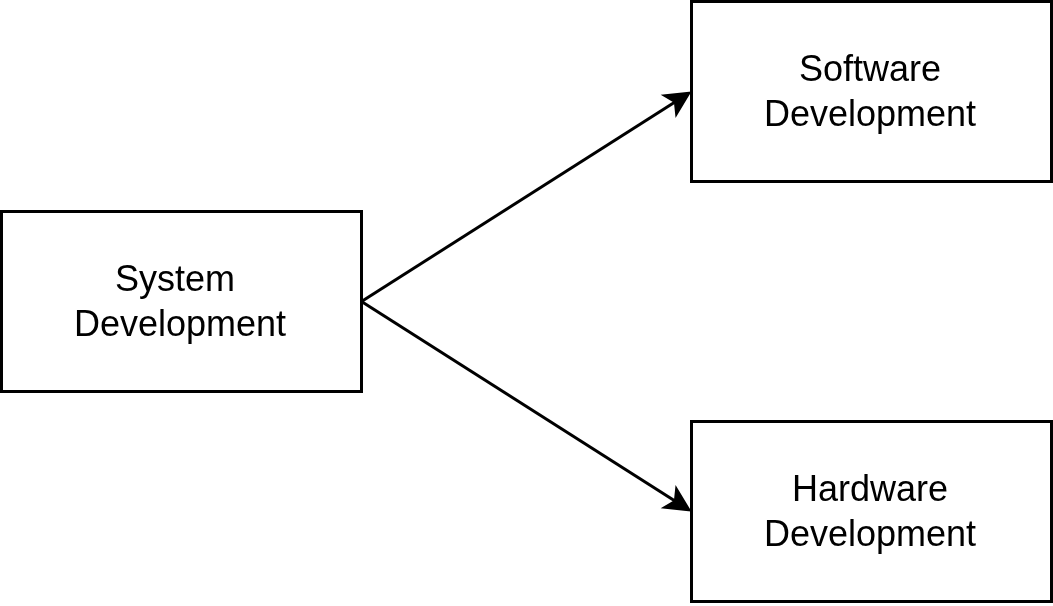
\includegraphics[width=0.4\textwidth]{sys.png} 
\end{figure}


\vspace{0.15cm}

\subsection{Software Crisis}
\begin{prettyBox}{Software Crisis}{myblue}
    Even though hardware became more abundant and available, creating software was still difficult because projects 
    could not be delivered on time, often went over budget, and were filled with bugs. This is what we call the 
    software crisis, and it was mainly due to a lack of methodology in software development.
\end{prettyBox}

\vspace{0.15cm}
\begin{center}
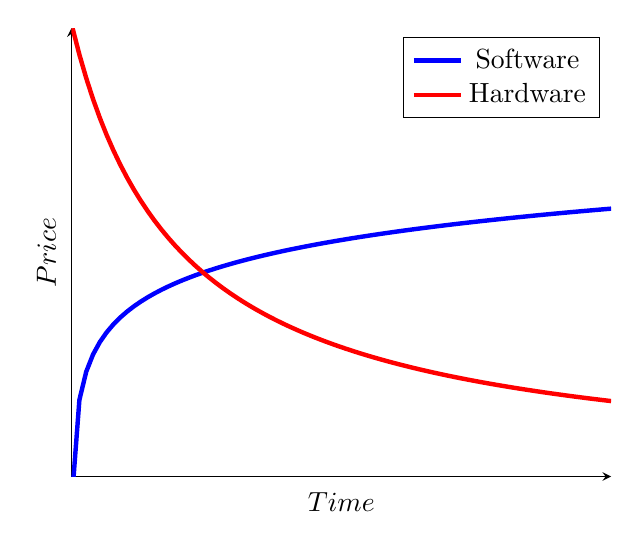
\begin{tikzpicture} 
\begin{axis}[ axis lines = left,
              xlabel=$Time$, 
              ylabel=$Price$, 
              domain=0.01:5, 
              xtick=\empty, 
              ytick=\empty, 
              xmin=0,
              ymin=0] 
\addplot[ultra thick, color = blue, no marks, samples = 80] {5 + ln(0.5*x)}; 
\addlegendentry{Software} 
\addplot[ultra thick, color = red, no marks, samples = 80] {10 / (x + 1)}; 
\addlegendentry{Hardware} 
\end{axis} 
\end{tikzpicture}
\end{center}

As shown in the graph above, there is an inverse relationship between hardware and software prices. As hardware becomes
more affordable and advanced, software prices tend to increase.

\newpage

\subsection{Life Cycle}
\begin{prettyBox}{Life Cycle}{myblue}
    The way we develop software is very important. To address the software crisis, engineers developed life cycles, which are 
    methodologies that help build software through chronological steps. One of the first life cycles still being used is the 
    waterfall life cycle. 
    
    Furthermore, system problems are divided into smaller, more manageable subproblems called modules, then linked together 
    (architectural design), and each module is then detailed (detailed design).
\end{prettyBox}


\begin{figure}[H]
  \begin{subfigure}[H]{.2\textwidth}
    \centering
    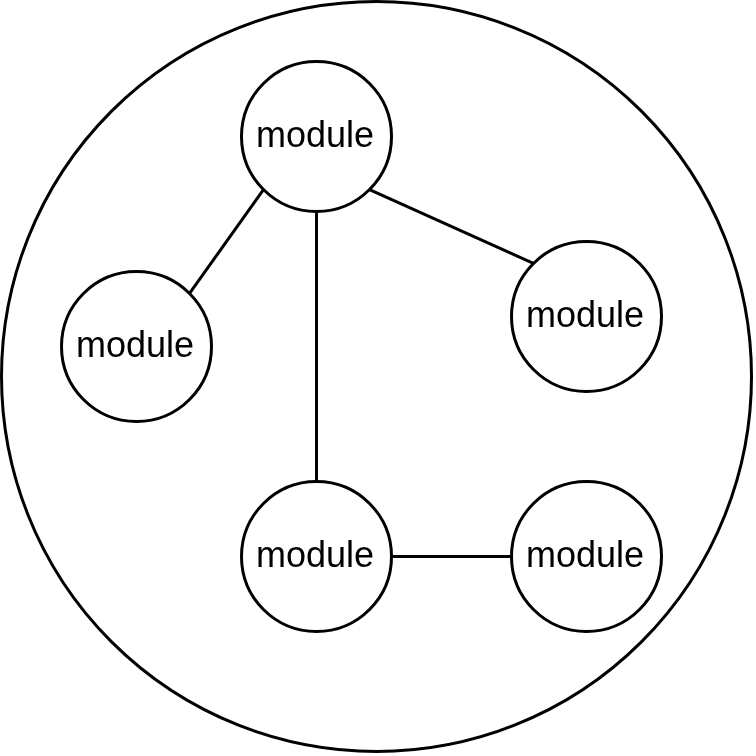
\includegraphics[width=\linewidth]{archi.png}
    \caption*{Architectural Design}
  \end{subfigure}
  \hfill
  \begin{subfigure}[H]{.6\textwidth}
    \centering
    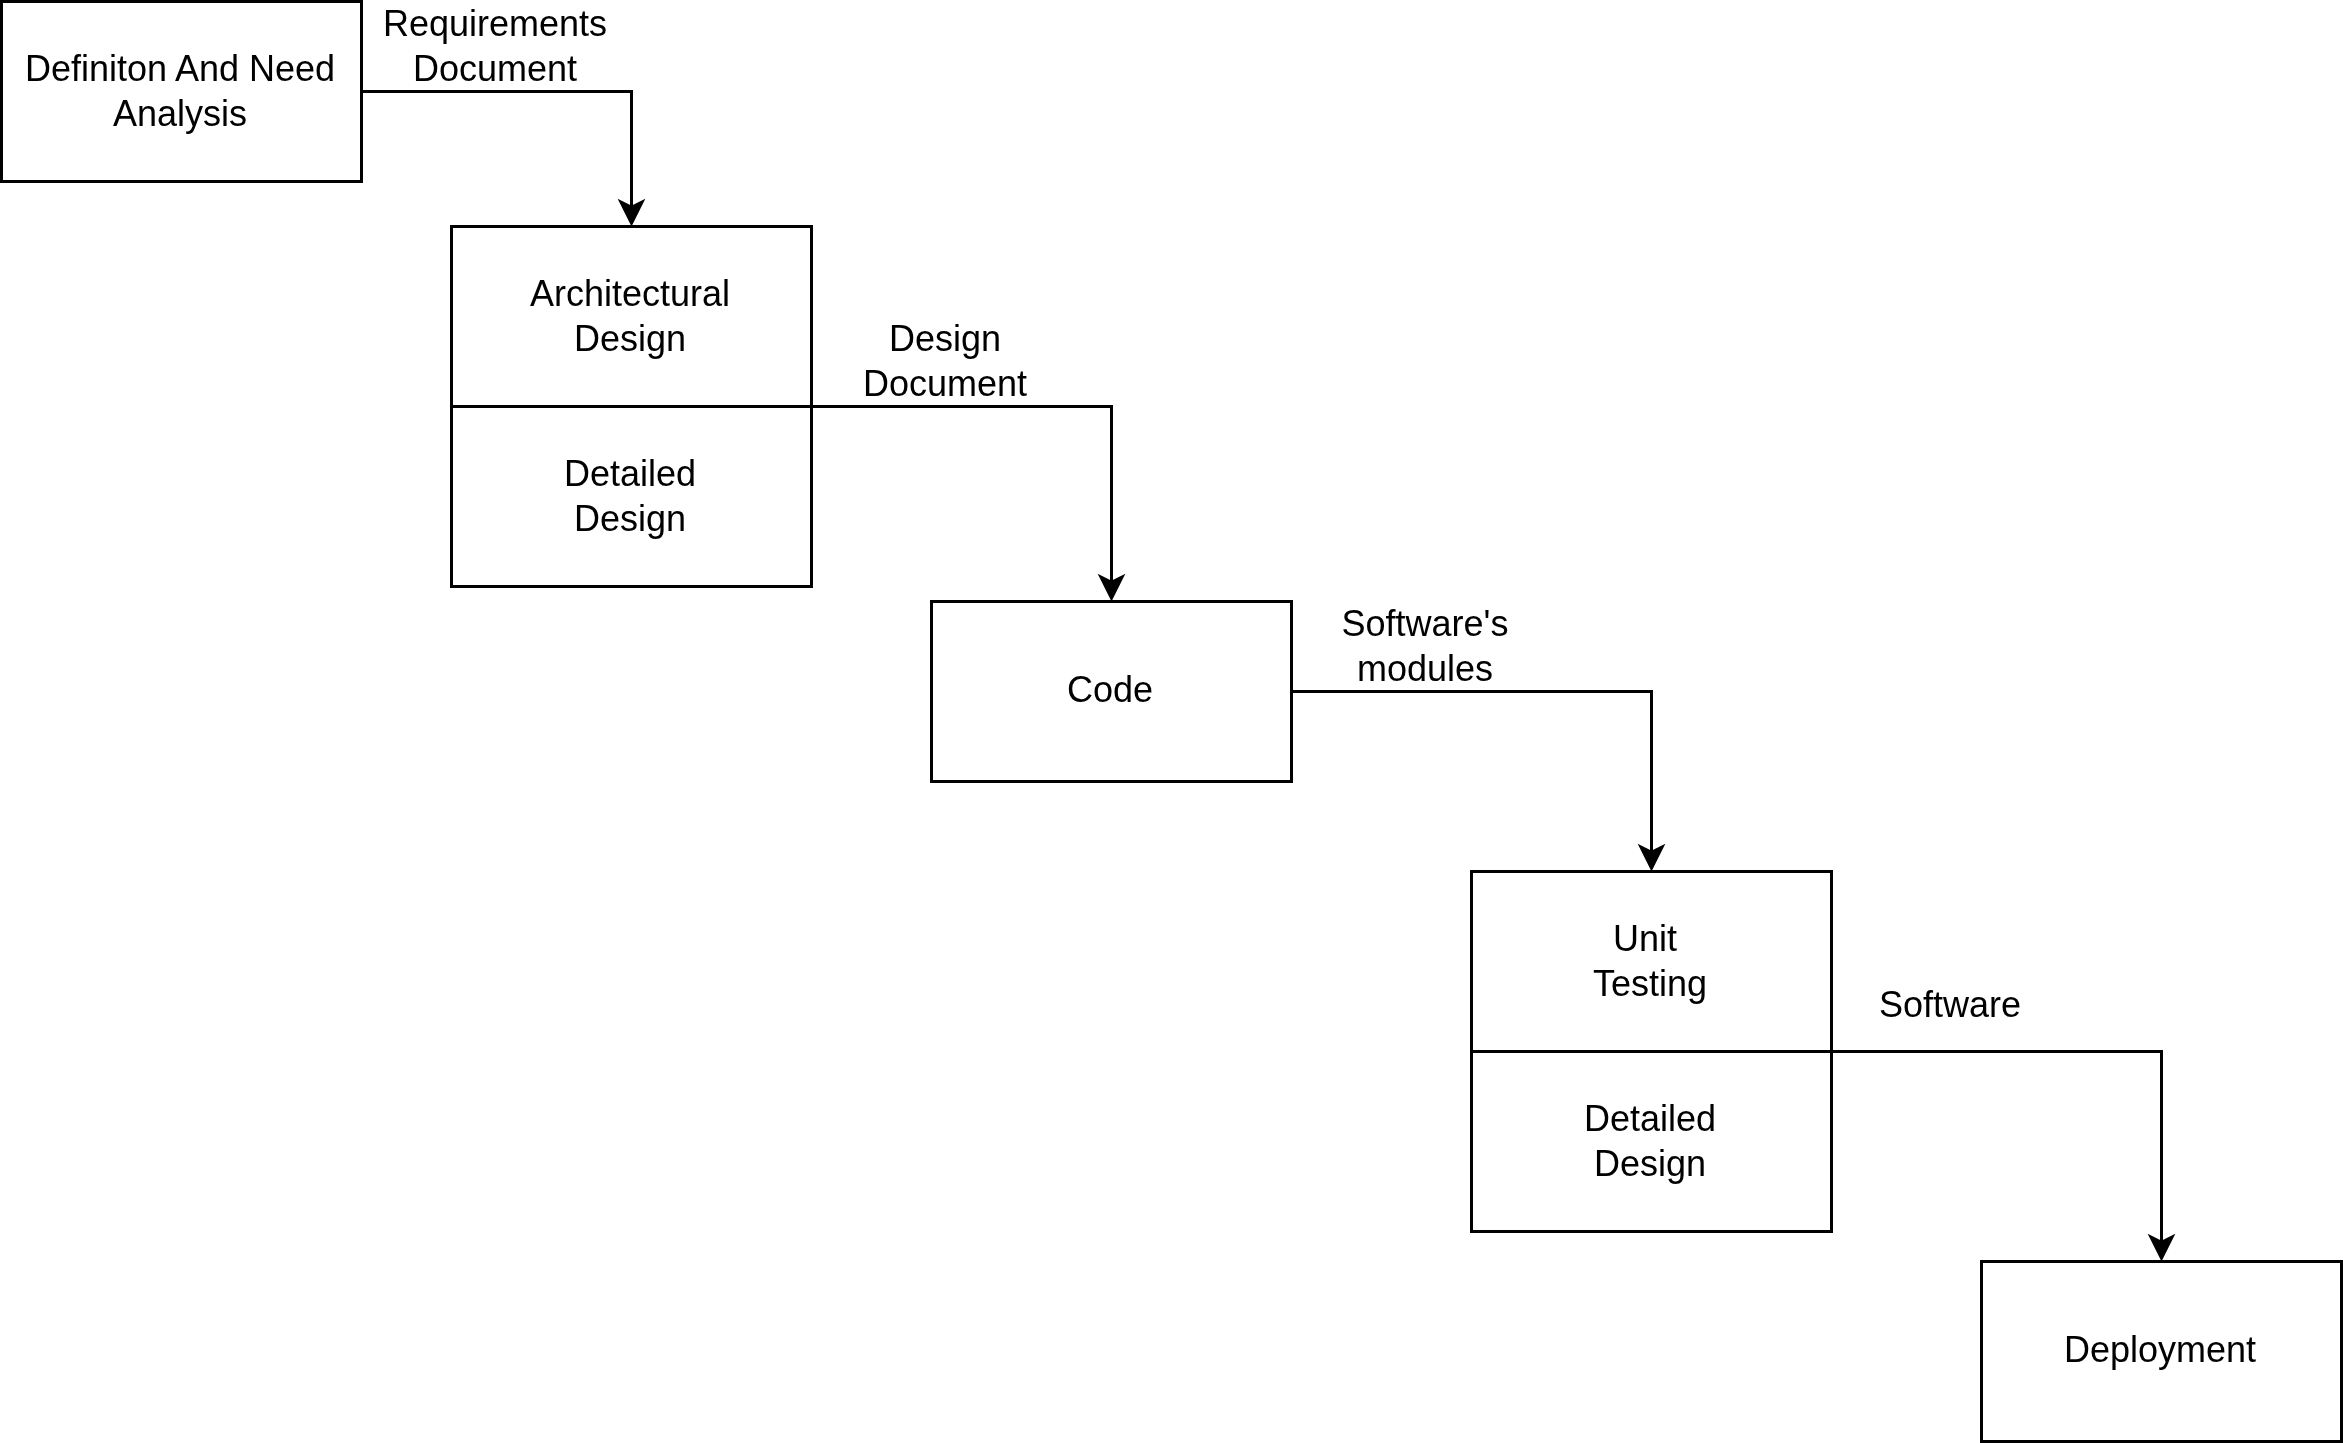
\includegraphics[width=\linewidth]{water.png}
    \caption*{WaterFall Life Cycle}
  \end{subfigure}
\end{figure}

\vspace{0.15cm}

\subsection{Process Management}
\begin{prettyBox}{Process Management}{myblue}
    In the 1980s, there was a growing interest in process management across many fields, e.g., how to organize medical processes in hospitals. With this came the ISO 9000 standard
    in 1987 to frame quality management regardless of the field.

    Therefore, software engineers started to create standards specific to software quality.
\end{prettyBox}

\vspace{0.15cm}

\subsection{Why Life Cycles Aren't Enough?}
\begin{prettyBox}{Why Life Cycles Aren't Enough?}{myblue}
    Even though life cycles provide a methodology, they are a bit too abstract and not detailed enough, e.g., how to go from architectural design 
    to detailed design? How should tasks be organized? etc.
\end{prettyBox}

\vspace{0.15cm}

\section{Type Of Software Process}
\begin{prettyBox}{Type}{myblue}
    The complexity of the process is tied to the complexity of the project, so we need to choose according to the context of the project. With
    hardware becoming more abundant, software became smaller, and from this came lighter processes such as Agile. In total, there are three types of processes:

    \begin{itemize}
        \itemsep0em 
        \item \textbf{Light-weight}: Agile
        \item \textbf{Heavy-weight}: classical processes
        \item \textbf{Hybrid}: use heavy-weight processes for complex phases and light-weight ones for simpler phases
    \end{itemize}
\end{prettyBox}


\begin{prettyBox}{Note}{red}
    \begin{itemize}
        \itemsep0em 
        \item Any organization uses processes wether implicit or explicit but we are only interested in explicits one. 
        \item Agile isn't magical solution for every project it has its limitation like any other process (not suited for critical project, works only
            for small teams, ...etc)
    \end{itemize}
\end{prettyBox}


\vspace{0.15cm}

\section{Examples Of Software Processes}
\begin{prettyBox}{Examples}{myblue}
    \begin{itemize}
        \itemsep0em 
        \item \textbf{Agile in the Large}: Agile methods applied to large, complex projects.
        \item \textbf{Global \& Distributed Software Processes}: divide a project into subprojects, each managed independently by different teams, often distributed geographically. The main challenges are communication and integration between subprojects.
        \item \textbf{Following the Sun (Around the Clock)}: similar to distributed development, but teams are organized across time zones so that work continues continuously, 24/7.
    \end{itemize}
\end{prettyBox}

\vspace{0.25cm}

\section{Configuration Software Rather Than Development}
\begin{prettyBox}{Configuration Software Rather Than Development}{myblue}
    Let freedom to user to configure the software, to turn off/on features and to change parameters to abide to a wider clientele like ERP.
\end{prettyBox}

\vspace{0.25cm}

\section{Software Processes \& Software Development}
\begin{prettyBox}{Definition}{myblue}
    Software development is a complexe task consisting of many inidvidual activities that need to be coordinated and this is where software
    processes come into place providing an infrastructure to coordinate \& manage these various activities
\end{prettyBox}

\vspace{0.1cm}
\begin{prettyBox}{Note}{red}
    If development organization doesn't explicitly define its process it still uses them at least implicitly.
\end{prettyBox}

\vspace{0.25cm}
\section{Why Use Software Process?}
\begin{prettyBox}{Why Use Software Process?}{myblue}
    \begin{itemize}
        \itemsep0em 
        \item simplification of understanding \& communication between organizations
        \item support process improvement
        \item support processes management
        \item automate execution of some tasks
        \item automate process guidance
        \item using defined process makes us more reliable and trustworthy for the client
        \item a means to convince third parties of the quality of the software (good quality software process leads to good quality software)
        \item process for risk management
        \item process in small development effort
        \item standardization of processes: follow the norms \& standards for guaranteed process quality
        \item industry \& technologies trends :
            \begin{itemize}
                \itemsep0em 
                \item \textbf{pros}: trends always bring something new 
                \item \textbf{cons}: we need to adapt the process accordingly
            \end{itemize}
        \item big organizations use them explicitly but smaller ones we use really simple process to not encumber and make development harder
        \item We have to adapt the processes to the risk management.
    \end{itemize}
\end{prettyBox}

\vspace{0.1cm}

\begin{prettyBox}{Conclusion}{red}
    Software processs variety changes according to context, complexity, standards followed, risk management, trends which complicate
    the management of the processes so this is why we have a field called \textbf{software processes}
\end{prettyBox}

\vspace{0.25cm}

\section{Defined \& Performed Process}

\subsection{Defined Process}
\begin{prettyBox}{Defined Process}{myblue}
    It's \textbf{theoritical ideal process} defining all activities, technologies while following the standards.
\end{prettyBox}

\vspace{0.15cm}
\subsection{Performed Process}
\begin{prettyBox}{Performed Process}{myblue}
    What we actually \textbf{apply in real life} we have constraints, sometimes people don't 100\% follow the process, 
    they may have a missunderstanding, or they don't do their work properly
\end{prettyBox}

\vspace{0.15cm}
\begin{prettyBox}{Note}{red}
    The performed process can never be 100\% identical to the defined process, we try to minimize the cost by continuous control.
\end{prettyBox}

\vspace{0.25cm}

\section{Process Selection \& Tailoring}
\begin{prettyBox}{Process Selection \& Tailoring}{myblue}
    \begin{itemize}
        \item \textbf{Process Selection}: select the appropriate process according to the context.
        \item \textbf{Process Tailoring}: adapt the process so it fits 100\%.
    \end{itemize}
\end{prettyBox}

\vspace{0.25cm}

\section{Process \& Product Quality}
\begin{prettyBox}{Process \& Product Quality}{myblue}
    A \textbf{good process leads to a good product/context} , but sometimes a good process used in project A 
    produced a good product but if used in another project B it \textbf{might not give as good of a result as A}. 
\end{prettyBox}

\vspace{0.25cm}
\section{Software Process Improvement (Continious)}

\subsection{Software process \& Knowledge Management}
\begin{prettyBox}{Software process \& Knowledge Management}{myblue}
 Knowledge gained from projects can be used to improve the software process.
\end{prettyBox}

\vspace{0.15cm}
\subsection{Software Process \& People}
\begin{prettyBox}{Software Process \& People}{myblue}
The process depends on the human factor, and humans are not predictable (motivation, creativity, etc.), which influences the process.
\end{prettyBox}

\vspace{0.15cm}
\subsection{Process (Broadly Speaking)}
\begin{prettyBox}{Process ISO 9000 Definition}{myblue}
    a set of interlaced or interacting activities which use inputs to deliver an intended result.
\end{prettyBox}


\vspace{0.15cm}
\subsection{Task}
\begin{prettyBox}{Task ISO 12207 Definition}{myblue}
    Required , recommanded or permissible action intended to contribute to the achievement of one 
    or more outcomes of a process
\end{prettyBox}

\vspace{0.15cm}
\subsection{Activity}
\begin{prettyBox}{Activity ISO 12207 Definition}{myblue}
    a set of cohesive tasks of a process
\end{prettyBox}

\vspace{0.15cm}
\subsection{Sub-Process}
\begin{prettyBox}{Sub-Process CMMI Definition}{myblue}
    a process that is part of a larger process
\end{prettyBox}

\vspace{0.15cm}
\subsection{Process Model}
\begin{prettyBox}{Process Model}{myblue}
    Description of a model.
\end{prettyBox}

\subsection{Process Instance}
\begin{prettyBox}{Process Instance ISO 33001 Definition}{myblue}
    Single specific \& identifiable execution of a process
\end{prettyBox}

\vspace{0.15cm}
\subsection{Role}
\begin{prettyBox}{Role}{myblue}
    A set of qualification and responsibilities played by actors (human , software , AI ...etc), on actor may
    play multiple roles at the same time.
\end{prettyBox}

\vspace{0.15cm}
\subsection{Product (Artifact)}
\begin{prettyBox}{Product PMBOK Definition}{myblue}
    That is produced is quantifiable and can be either an end item in itself or a componant item
\end{prettyBox}

\vspace{0.15cm}
\section{Model (Broadly Speaking)}
\begin{prettyBox}{Model}{myblue}
    Abstract representation of an existing entity or an entity to be created.
\end{prettyBox}

\vspace{0.25cm}

\section{Type Of Model}
\subsection{Descriptive \& Prescriptive Model}
\begin{prettyBox}{Descriptive \& Prespective Model}{myblue}
    \begin{itemize}
        \item \textbf{Descriptive Model} : if a model represents an \textbf{existing entity} , e.g : biology describes existing creatures.
        \item \textbf{Prescriptive Model} : if it represents an \textbf{entity to be created} , e.g : blueprint of building prescribes an entity to be created.
    \end{itemize}
\end{prettyBox}

\vspace{0.15cm}
\subsection{Difference Between Descriptive \& Prescriptive Model}
\begin{prettyBox}{Difference}{red}
    The difference resides solely in the \textbf{purpose but not necessarily in the content} of the model.
\end{prettyBox}


\vspace{0.25cm}
\section{Software Process Model}
\begin{prettyBox}{Software Process Model}{myblue}
    \begin{itemize}
        \item \textbf{Describes The Way Software Is To Be Developed} : in this case the software doesn't exist already
            therefore it's a \textbf{prescriptive model} to design the entity to be created.
        \item \textbf{Describes How The Software Is Actually Developed} : the software already exists so it's a\\ 
            \textbf{descriptive model}, its purpose is to \textbf{analyse \& improve this process}.
    \end{itemize}
\end{prettyBox}

\vspace{0.15cm}

\begin{prettyBox}{Note}{red}
    Software processes have the property of utilizing both descriptive \& prescriptive models.
\end{prettyBox}


\vspace{0.25cm}

\section{Stachowiak's General Model Theory (GMT)}
\begin{prettyBox}{GMT}{myblue}
In this theory the model is characterized by 3 properties :
    \begin{itemize}
        \item \textbf{Mapping Property} : a model is \textbf{mapping or representation} of some entity.
        \item \textbf{Reduction Property} : a model is a \textbf{reduction of the represented entity} and 
            \textbf{doesn't contain all attributes} of the original (\textbf{an abstraction}).
        \item \textbf{Pragmatic Property} : a model is created for a \textbf{certain purpose} which implies that 
            \textbf{the perfect model doesn't exist}, moreover one entity \textbf{may have different models} each 
            contributing to a different purpose e.g building blueprints : architectural (layout/design), structural (foundation/framing), MEP (mechanical, electrical, plumbing).
    \end{itemize}    
\end{prettyBox}

\vspace{0.25cm}

\section{Meta Model}

\begin{prettyBox}{Meta Model}{myblue}
    In order to describe a model we need to define \textbf{how is to be done} and what {terminologies} may be 
    used, in other words we need a model for the model (a meta model).
\end{prettyBox}


\vspace{0.25cm}

\section{ISO Meta Model Definition}
\subsection{ISO 24744}
\begin{prettyBox}{ISO 24744}{myblue}
    Meta model is specification of the concept relationships on the rules that are used to define a mythodology.
\end{prettyBox}

\vspace{0.15cm}
\subsection{ISO 15909}
\begin{prettyBox}{ISO 15909}{myblue}
    Meta model is a model defining the concept and the relation for some modeling notation.
\end{prettyBox}


\vspace{0.25cm}
\section{Simple Example Of Meta Model}

\begin{figure}[H] 
  \centering 
  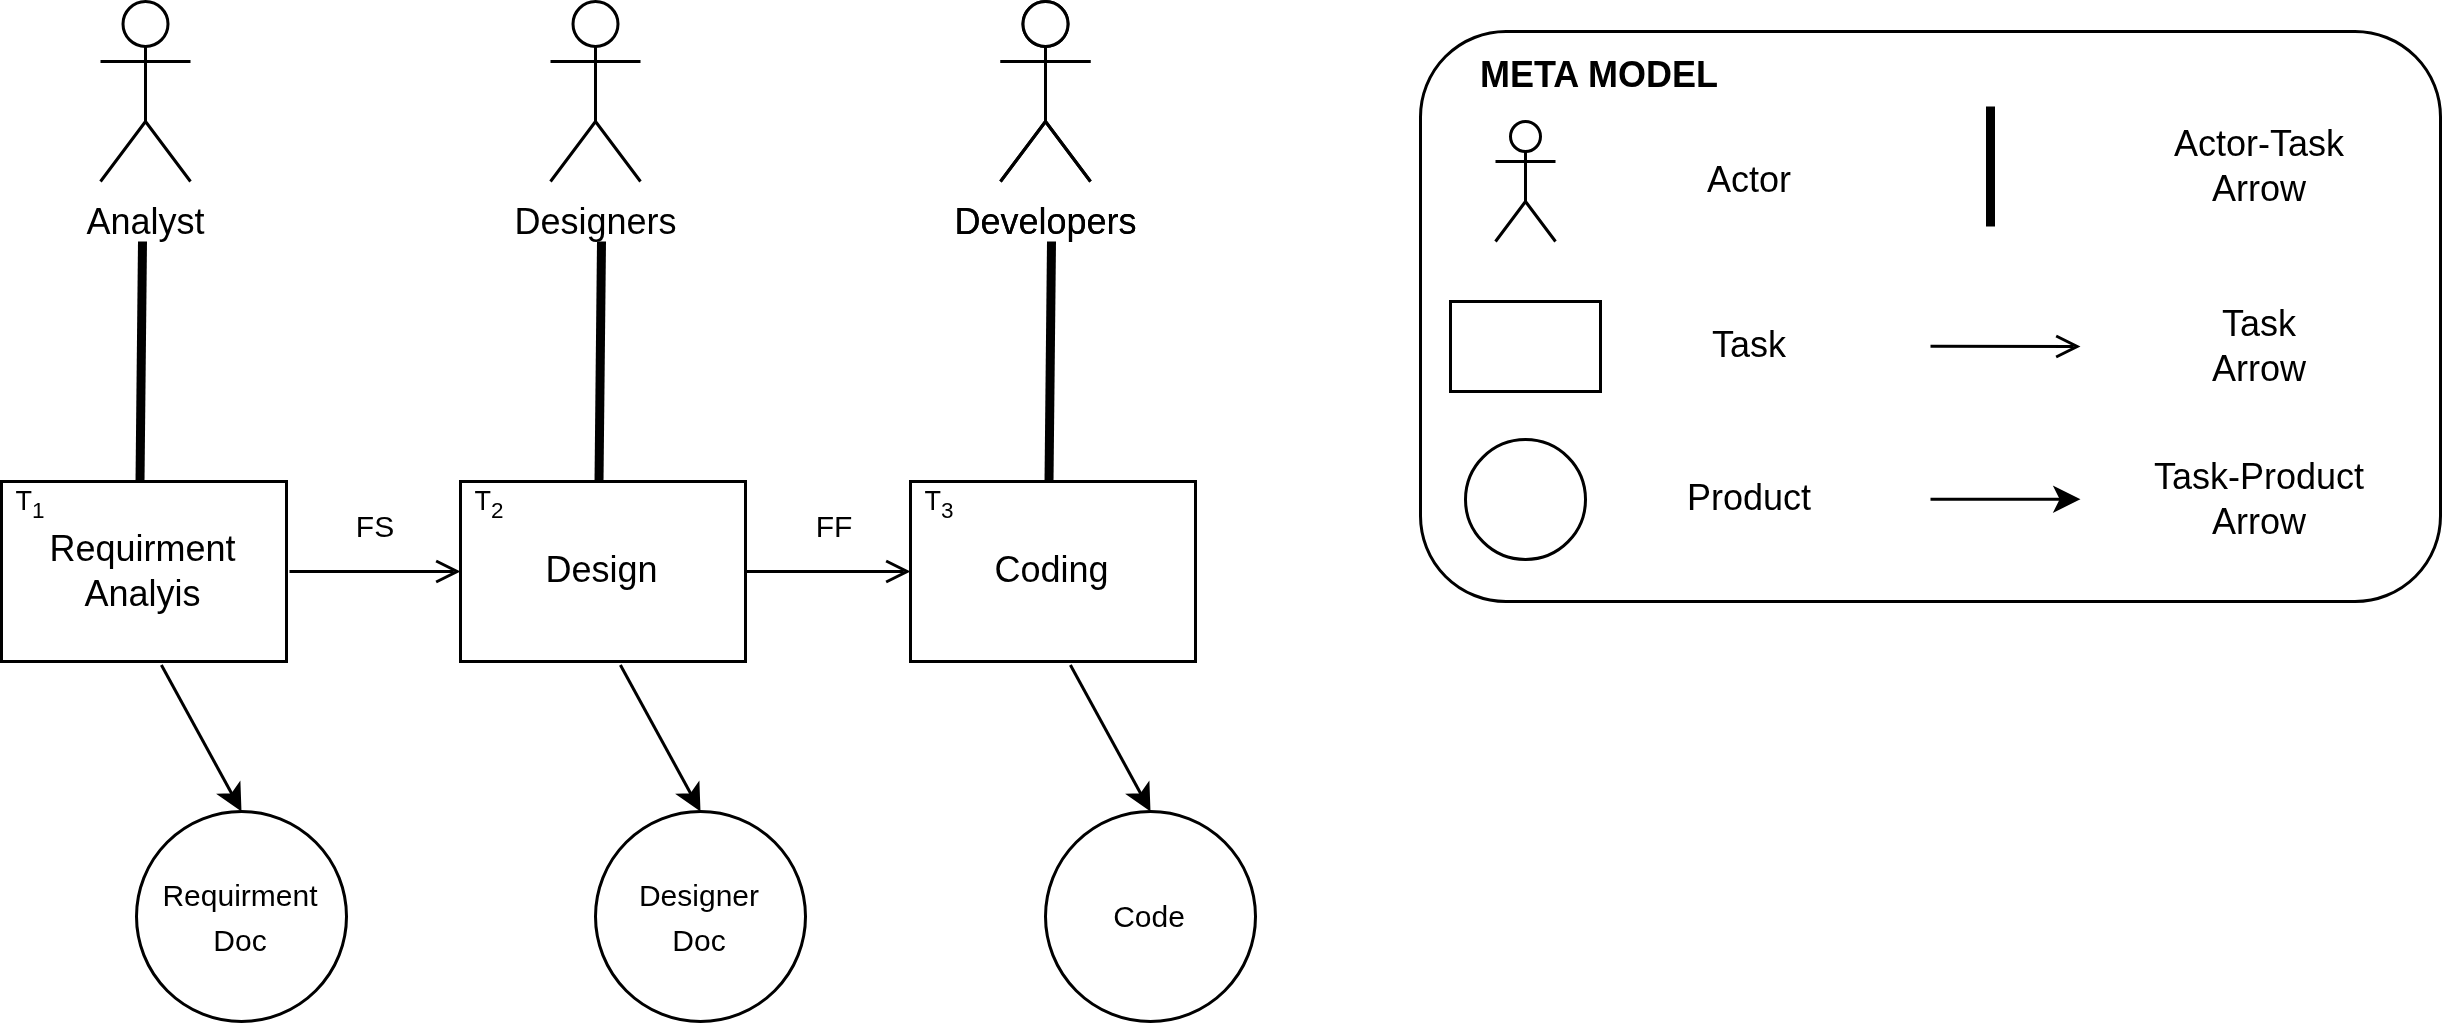
\includegraphics[width=0.6\textwidth]{meta.png} 
\end{figure}

\end{document}
